\section{面谈}

\subsection{概述}
\begin{itemize}
    \item 面对面的会见(face-to-face meeting)被认为是最具丰富内容的交流方法
    \item 实践当中应用最为广泛的需求获取方法之一 
    \item 可以获得的信息内容包括 
    \vspace{-0.8em}
	\begin{multicols}{2}
    \begin{itemize}
        \item 事实和问题 
        \item 被会见者的观点 
        \item 被会见者的感受 
        \item 组织和个人的目标 
    \end{itemize}
	\end{multicols}
\end{itemize}

\begin{figure}[H]
	\centering
	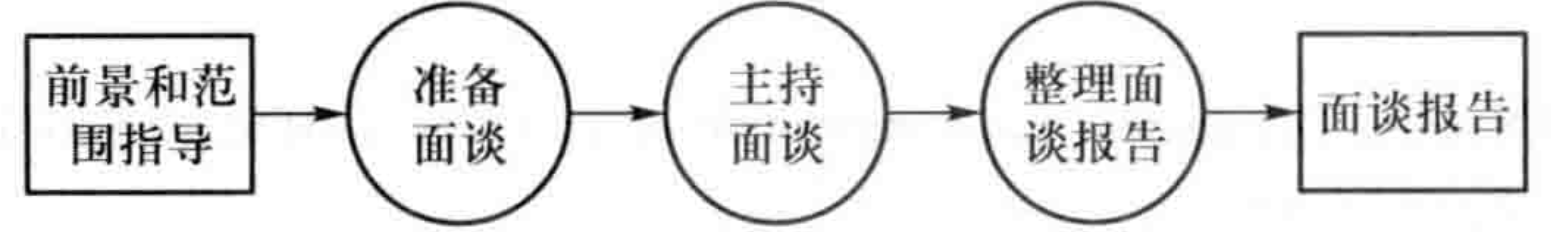
\includegraphics[width=0.6\textwidth]{img/面谈的基本过程.png}
    \caption*{面谈的基本过程}
    \vspace{-1em}
\end{figure}

\subsection{准备面谈}

\subsubsection{准备工作}
面谈淮备的主要工作包括以下几方面
\vspace{-0.8em}
\begin{multicols}{2}
    \begin{itemize}
        \item 阅读背景资料 
        \item 确定面谈主题和目标 
        \item 选择被会见者 
        \item 通知被会见者:电话或邮件等正式的途径 
        \item 确定问题和类型   
    \end{itemize}
\end{multicols}
\vspace{-1em}

\subsubsection{问题类型}
准备问题不仅仅是要清楚面谈的内容,更要清楚提问题的方法,尤其是要恰当地使用各种不同问题类型
\vspace{-0.8em}
\begin{multicols}{4}
    \begin{itemize}
        \item 开放式问题
        \item 封闭式问题
        \item 程序性提示 
        \item 探究式问题
        \item 诱导式问题
        \item 元问题
        \item ……
    \end{itemize}
\end{multicols}
\vspace{-1em}

问题基本上可以分为两种类型:开放式问题和封闭式问题

\textbf{开放式问题} \par
被会见者对答复的选择可以是开放和不受限制的,他们可能答复两个词,也可能答复两段话

在希望得到丰富(具有一定深度和广度)信息时,开放式问题比较合适

开放式问题举例
\vspace{-0.25em}
{\kaishu \begin{compactitem}
    \item “你觉得把所有的经理都置于一个内联网内怎么样?”
    \item “请解释你是如何做进度决策的?”
    \item “对公司中企业对企业电子商务的当前状态有何看法?”
\end{compactitem}}

开放式问题的优点
\begin{itemize}
    \item 让被会见者感到自在;
    \item 会见者可以收集被会见者使用的词汇,这能反应他的教育、价值标准、态度和信念;
    \item 提供丰富的细节;
    \item 对没采用的进一步的提问有启迪作用;
    \item 让被会见者更感兴趣;
    \item 容许更多的自发性;
    \item 会见者可以在没有太多准备的情况下进行面谈。
\end{itemize}

开放式问题的缺点
\begin{itemize}
    \item 提此类问题可能会产生太多不相干的细节;
    \item 面谈可能失控;
    \item 开放式的回答会花费大量的时间才能获得有用的信息量;
    \item 可能会使会见者看上去没有准备。
\end{itemize}

\textbf{封闭式问题} \par
答案有基本的形式,被会见者的回答是受到限制的 

封闭式问题举例
\vspace{-0.25em}
{\kaishu \begin{compactitem}
    \item “项目存储库每个星期更新多少次?”
    \item “电话中心一个月平均收到多少个电话?”
    \item “下列信息中哪个对你最有用:(1)填好的客户投诉单;(2)访问web站点的客户的电子邮件投诉;(3)与客户面对面的交流;(4)退回的货物。”
    \item “列出头两项需要优先考虑的改善技术基础设施的事项。”
\end{compactitem}}

封闭式问题的优点
\vspace{-0.8em}
\begin{multicols}{2}
    \begin{itemize}
        \item 节省时间
        \item 切中要点
        \item 保持对面谈的控制
        \item 快速探讨大范围问题
        \item 得到贴切的数据
    \end{itemize}
\end{multicols}
\vspace{-1em}

封闭式问题的缺点
\vspace{-0.8em}
\begin{multicols}{2}
    \begin{itemize}
        \item 使得被会见者厌烦
        \item 得不到丰富的细节
        \item 出于上述原因,失去主要思想
        \item 不能建立和面谈者的友好关系
    \end{itemize}
\end{multicols}
\vspace{-1em}

\textbf{程序性提示} \par
程序性提示是针对一些人的思维特点而设计的面谈问题[Pitts 2007],它们的使用是程序性的,也就是说到了特点的面谈程序点,就应该使用相应的程序性提示问题。

\begin{table}[H]
    \centering
    \begin{tabular}{|c|l|}
    \hline
    提示                         & \multicolumn{1}{c|}{示例}                                                           \\ \hline
    \multirow{3}{*}{总结和反馈}     & 你能不能总结一下系统的功能?                                                                    \\ \cline{2-2} 
                               & 你能不能总结一下一个成功系统的必备特征?                                                              \\ \cline{2-2} 
                               & 在使用的时候,你希望能够从系统当中得到什么类型的信息反馈?                                                     \\ \hline
    \multirow{3}{*}{重复和改述}     & 能不能再说一次系统的哪些特征是重要的?                                                               \\ \cline{2-2} 
                               & 你能不能详细的重新叙述一下使用系统的步骤?                                                             \\ \cline{2-2} 
                               & 在使用系统的时候你会做出什么决定?                                                                 \\ \hline
    \multirow{3}{*}{建立场景和细节描述} & 有什么是你现在能做,却在新系统中不能做的?                                                             \\ \cline{2-2} 
                               & 在什么情况下,功能是必需的?                                                                    \\ \cline{2-2} 
                               & \begin{tabular}[c]{@{}l@{}}设想现在是6个月之后,你需要评估系统的成功状况,你会使用哪\\ 些标准来做出评价?\end{tabular} \\ \hline
    \multirow{3}{*}{抗辩}        & 你能不能想出什么不使用系统的理由?                                                                 \\ \cline{2-2} 
                               & 你为什么会不想使用系统呢?                                                                     \\ \cline{2-2} 
                               & 你能不能想出将来可能导致系统失败或故障的原因?                                                           \\ \hline
    \end{tabular}
\end{table}
\vspace{-0.5em}

\textbf{其他重要的问题类型} \par
\begin{itemize}
    \item 探究式问题
    \vspace{-0.25em}
    {\kaishu \begin{compactitem}
    \item 为什么?
    \item 你能举个例子吗?
    \item 你能详细描述一下吗?
    \end{compactitem}}
    \item 诱导性问题
    \vspace{-0.25em}
    {\kaishu \begin{compactitem}
    \item “你和其他经理一样,都同意把财产管理计算机化,是吗” 
    \end{compactitem}}
    \item 双筒问题
    \vspace{-0.25em}
    {\kaishu \begin{compactitem}
    \item “每天你通常会做什么决策,你是怎样做的” 
    \end{compactitem}}
    \item 元问题
    \vspace{-0.25em}
    {\kaishu \begin{compactitem}
    \item 我的问题看起来相关吗?
    \item 你的回答正式吗?
    \item 你是回答这些问题的最佳人选吗?
    \item 我问了太多的问题吗?
    \item 我还应该见什么人? 
    \end{compactitem}}
\end{itemize}


\subsubsection{问题准备}
\vspace{-0.8em}
\begin{multicols}{2}
\columnseprule=0.8pt
需求工程前期
\begin{itemize}
    \item 开放式问题为主
    \item 决策层与专家为主
    \item 遵循问题$\rightarrow$目标$\rightarrow$解决方案路线
    \begin{itemize}
        \item 问题、目标
        \item 目标、任务(流程$\rightarrow$任务)
    \end{itemize}
    \item 分析基本的涉众特点
    \begin{itemize}
        \item 角色、任务、个人目标、频率、优先级
    \end{itemize}
\end{itemize}

需求工程后期
\begin{itemize}
    \item 封闭式问题为主
    \item 抓住主题与线索,例如,任务分解、流程图、界面示意等
    \item 问题针对性
    \begin{itemize}
        \item 任务分解关系
        \item 流程正确性、异常
        \item 界面中的行为、数据项
    \end{itemize}
    \item 事先准备面谈记录材料
\end{itemize}
\end{multicols}
\vspace{-1em}

面谈的问题准备示例一

{\kaishu
(面谈对象:投资人、管理者)
\vspace{-0.25em}
\begin{compactenum}[1.]
    \item 目前的业务主要碰到了哪些问题?\\
    (预计:销售效率低;积压、缺货、报废现象严重;成本较高;竞争力不足)
    \item 希望新系统能够帮助达成哪些目标?\\
    (预计:提高销售效率;减少积压、缺货、报废现象;降低成本;提高竞争力;提升销售额)\\
    (如果存在销售效率问题)
    \item 销售工作是怎样进行的?
    \item 哪些人会参与销售过程?
    \item 哪些人的哪些工作是最为瓶颈的?
\end{compactenum}
\vspace{-0.5em}
……}

面谈的问题准备示例二

{\kaishu
(面谈对象:投资人、管理者)
\vspace{-0.25em}
\begin{compactenum}[1.]
    \item 销售人员的主要工作是什么?\\
    (预计:销售处理、退货处理)
    \item 销售处理的主要过程是怎样的?
    \item 销售处理工作目前的困难有哪些?
    \item 销售处理的频率怎么样?
    \item 平均多长时间完成一次销售处理?
\end{compactenum}
\vspace{-0.5em}
……}

面谈的问题准备示例三
\vspace{-0.8em}
{\kaishu
\begin{multicols}{2}
    用例/场景描述
    \vspace{-0.25em}
    \begin{compactenum}[1.]
        \item 收银员输入会员编号;
        \item 系统显示会员信息;
        \item 收银员输入商品;
        \item 系统显示输入商品的信息;
        \item 系统显示所有已输入商品的信息;
    \end{compactenum}
    \vspace{-0.65em}
    收银员重复3$\sim$5步,直至完成所有输入
    \vspace{-0.6em}
    \begin{compactenum}[1.]
        \setcounter{enumi}{5}
        \item 收银员结束商品输入;
        \item 系统显示总价和赠品信息;
        \item 收银员请求顾客付款;
        \item 顾客支付,收银员输入支付数额;
        \item 系统显示应找零数额,收银员找零;
        \item 收银员结束销售;
        \item 系统更新数据,并打印收据。
    \end{compactenum}

    问题:
    \vspace{-0.25em}
    \begin{compactenum}[1.]
        \item 会员编号的格式是怎样的?
        \item 需要显示的会员信息有哪些?
        \item 商品是怎样输入的?
        \item 需要显示的商品信息有哪些?
        \item 系统应该怎样显示已输入商品的信息?
        \\
        \item 总价是怎样计算的?
        \item 需要显示的赠品信息有哪些?
        \item 收据的格式是怎样的?
        \item 有可能不输入会员编号吗?
        \item 有可能不输入商品吗?
        \item 有可能不结束销售吗?
        \item 付款时有其他非现金方式吗?
    \end{compactenum}   
\end{multicols}
\vspace{-1em}}

\subsubsection{面谈背后的要点:取得“共情”与“目标”的平衡}
共情
\vspace{-0.8em}
\begin{multicols}{2}
    \begin{itemize}
        \item 取得信任
        \item 激发主动性
        \item 获得更全面的问题域背景(主观)和业务意向(个人)
        \item 客户洞察:功能$\rightarrow$认知$\rightarrow$情感;面谈可视作“反向的客户洞察”
    \end{itemize}
\end{multicols}
\vspace{-1em}

目标
\vspace{-0.8em}
\begin{multicols}{2}
    \begin{itemize}
        \item 充分、正确地获取用户需求
        \item 在项目前景和范围指导下充分获取用户需求与问题域知识
        \item 利用开放式问题、探究式问题和程序性提示增强覆盖范围
        \item 利用封闭式问题确认细节
        \item 主动控制面谈过程
    \end{itemize}
\end{multicols}
\vspace{-1em}


\subsection{主持面谈}
在面谈之前的注意事项
\vspace{-0.8em}
\begin{multicols}{2}
    \begin{itemize}
        \item 记得和被会见者联系并确认面谈的安排
        \item 着装正式
        \item 不要迟到
        \item 表现出来你已经准备好参加面谈了
    \end{itemize}
\end{multicols}
\vspace{-1em}

实际的面谈分为3个阶段:开始、主体和结束
\begin{itemize}
    \item 开始:建立一个理想的氛围和环境来促进会见者和被会见者之间的交流和沟通 
    \item 主体:通过提问和倾听来完成和被会见者的信息交流,按照计划控制面谈的进行,并在必要时进行适当的调整 
    \item 结束:表示感谢并回答被会见者提出的问题。保持与被会见者的亲善和信任关系 
\end{itemize}

\subsubsection{面谈开始阶段}
面谈开始阶段需要注意的事项包括:
\vspace{-0.8em}
\begin{multicols}{2}
    \begin{itemize}
        \item 开场仪式:握手
        \item 简要重申面谈的目标
        \item 准备好笔记本、录音机或者其他记录设备
        \item 用一些一般的、轻松的、开放式的问题为开始
    \end{itemize}
\end{multicols}
\vspace{-1em}

\subsubsection{面谈主体阶段}
面谈主体阶段的注意事项包括以下几方面:
\begin{itemize}
    \item 保持有礼貌的倾听:遵循交流模式
    \item 控制面谈过程:主动打破交流模式
    \item 保持面谈主题:以面谈问题为主线索
    \item 使用探究式问题 
    \item 观察被会见者:在一个人的全部感觉中,只有7\%是通过口头(语言)交流的,38\%是通过语调交流的,55\%是通过面部表情和肢体语言交流的
    \item 使用道具支持
\end{itemize}

\subsubsection{面谈结束阶段}
面谈结束阶段的注意事项主要有以下几方面:
\begin{itemize}
    \item 面谈应该在45分钟到1小时内结束,并非要在提出所有关心的问题后才能结束面谈,相反,结束面谈应该比开始面谈更自然;
    \item 总结谈话的要点,如果有记录笔记的话可以请被会见者进行快速的检查,确保记录下了面谈的所有重要信息;
    \item 感谢被会见者,并且给时间让他们询问一些他们自己关心的问题;
    \item 握手话别。 
\end{itemize}

\subsubsection{处理面谈结果}
\vspace{-0.8em}
\begin{multicols}{2}
    \begin{itemize}
        \item 复查面谈记录:整理内容要点,进行分类 
        \item 总结面谈信息:评估面谈中所得到的信息 
        \item 完成面谈报告
    \end{itemize}
\end{multicols}
\vspace{-1em}

\subsection{面谈的类型}
\begin{itemize}
    \item 结构化面谈
    \begin{itemize}
        \item 完全按照事先的问题和结构来控制面谈 
    \end{itemize}
    \item 半结构化面谈
    \begin{itemize}
        \item 事先需要根据面谈内容准备面谈的问题和面谈结构,但在面谈过程当中,会见者可以根据实际情况采取一些灵活的策略
    \end{itemize}
    \item 非结构化面谈 
    \begin{itemize}
        \item 没有事先预定的议程安排,常见情况
        \item 甚至会在没有太多事前准备的情况下就直接到访被会见者的工作地,就某个主题开展会谈
        \item 会见者和被会见者谈话的主题可能非常广泛,而且每个主题都不会非常深入
        \item 也可能在非结构面谈中仅就某个特殊的主题进行深入的讨论
        \item 考验对领域的理解、面谈技巧、整理笔录等诸多能力
    \end{itemize}
\end{itemize}

\subsection{面谈的优点和局限性}
面谈的优点有:
\begin{itemize}
    \item 面谈的开展条件较为简单,经济成本较低;
    \item 能获得包括事实、问题、被会见者观点、被会见者态度和被会见者信仰等各种信息类型在内的广泛内容;
    \item 通过面谈,需求工程师可以和涉众(尤其是用户)建立相互之间的友好关系;
    \item 通过参与面谈,被会见者会产生一种主动为项目做出贡献的感觉,提高涉众的项目参与热情。  
\end{itemize}

面谈的缺点和局限性包括:
\begin{itemize}
    \item 面谈比较耗时,时间成本较高;
    \item 在被会见者地理分散的情况下往往难以实现面谈;
    \item 面谈参与者的记忆和交流能力对结果影响较大,尤其是面谈的成功较高的依赖于需求工程师的人际交流能力;
    \item 交谈当中常见的概念结构不同、模糊化表述、默认知识、潜在知识和态度偏见等各种问题在面谈中都不可避免,进而影响面谈的效果,导致产生不充分的、不相关的或者错误的数据;
    \item 在会见者不了解被会见者认知结构的情况下,面谈不可能取得令人满意的效果。
\end{itemize}

\subsection{和面谈相关的其他需求获取方法}

\subsubsection{群体面谈}
群体面谈的方法是将所有的涉众方集中起来,选择一个合适的地点,集中一段时间,召开一个多方共同参与的会议,一起进行需求的讨论、分析和获取。

群体面谈的需求获取方法
\vspace{-0.8em}
\begin{multicols}{2}
    \begin{itemize}
        \item 联合应用程序设计JAD
        \item 需求专题讨论会
        \item 需求中心小组
        \item 联合需求规划JRP
    \end{itemize}
\end{multicols}
\vspace{-1em}

群体面谈的优点:节约时间,有着更低的时间成本。

群体面谈的缺点:主持群体面谈比主持一对一面谈要困难的多。

群体面谈的三个阶段:计划面谈、主持面谈和分析结果
\begin{itemize}
    \item 计划面谈
    \begin{itemize}
        \item 确定参与人员:涉众、主持人、负责人、分析人员、记录人员、观察员
        \item 安排会谈时间:全职的2$\sim$4天参与会议,拟定一份议程
        \item 选择会谈地点:充足的空间,道具支持,良好的餐饮服务
        \item 准备会谈内容:面谈的主题和范围,会议的议程,需求的预期和会谈的目标,各种材料
    \end{itemize}
    \item 主持面谈
    \begin{itemize}
        \item 建立基本规则
        \vspace{-1em}
        \begin{multicols}{2}
        \begin{itemize}
            \item 按时开始和结束会议
            \item 中途休息(例如午餐)后要尽快进入状态
            \item 一次只讨论一个主题
            \item 期望每个人都为会议做出自己的贡献
            \item 要关注于问题,不要有人身批评和攻击
            \item 限制发言时间,不要个人把持会议   
        \end{itemize}
        \end{multicols}
        \vspace{-1em}
        \item 保持会议的气氛
        \item 确保每个人都积极地参与讨论
        \item 控制会议的主题
    \end{itemize}
    \item 分析结果
\end{itemize}

\subsubsection{调查问卷}
面谈方法以口头语言为主要的交流媒介,而调查问卷以文档为主要的交流媒介

适用调查问卷的情况
\begin{itemize}
    \item 系统的涉众在地理上是分布的;
    \item 系统的涉众数量众多,而且了解所有涉众的统计倾向是非常重要的;
    \item 需要进行一项探索性的研究,并希望在确定具体方向之前了解当前的总体状况;
    \item 为后续的面谈标识问题和主题,建立一个开展工作的基础框架。
\end{itemize}

调查问卷也是面谈
\vspace{-0.8em}
\begin{multicols}{2}
\begin{itemize}
    \item 适用于面谈的基本要求
    \item 留意内容导向
    \item 基于选择题的开放式问题与基于主观题的封闭式问题
\end{itemize}
\end{multicols}
\vspace{-1em}

\subsubsection{头脑风暴}
它的目的不是发现需求,而是“发明”需求,或者说是发现“潜在”需求

它鼓励参与者在无约束的环境下进行某些问题的自由思考和自由讨论,以产生新的想法 

适用情况
\vspace{-0.8em}
\begin{multicols}{2}
\begin{itemize}
    \item 发明并描述以前不存在的全新的业务功能
    \item 明确模糊的业务
    \item 在信息不充分的情况做出决策
\end{itemize}
\end{multicols}
\vspace{-1em}

头脑风暴通常包括两个阶段:想法产生阶段和想法精简阶段
\begin{itemize}
    \item 想法产生阶段
    \begin{itemize}
        \item 目的是产生出尽可能多的新的想法 
        \item 基本规则
        \begin{itemize}
            \item 充分发挥想像力,不要有任何的羁绊
            \item 产生尽可能多的想法,想法重在数量而不是质量,不要顾及想法是否荒诞
            \item 自由讨论,目的是产生新的想法,不要争吵和批评
            \item 在自由讨论当中,可以转换和组合所有已提出的想法,以产生新的想法 
        \end{itemize}
        \item 通常持续1个小时左右,特殊情况下持续$2\sim 3$个小时
    \end{itemize}
    \item 想法精减阶段
    \begin{itemize}
        \item 第一步是去除那些不值得进一步讨论的想法
        \item 第二步是把类似的意见进行归类
        \item 第三步是主持人遍历每一个未被删除的想法,确保所有参与者都对其有共同的理解
        \item 利用投票或类似方法,评估现有想法的优先级
        \item 最后,根据评估的数据,从中筛选出符合一定标准的想法作为头脑风暴方法的成果 
    \end{itemize}
\end{itemize}


